% Chapter Template

\chapter{Methodology} % Main chapter title

\label{Methodology} % Change X to a consecutive number; for referencing this chapter elsewhere, use \ref{ChapterX}

\lhead{Chapter \ref{Methodology}. \emph{Methodology}} % Change X to a consecutive number; this is for the header on each page - perhaps a shortened title

The thesis will utilize a design research methodology to perform its research. 
The guidelines provided in \citet{Hevner2004} will be followed to ensure that the process is rigorous.
The guidelines provided in this article are:
\begin{enumerate}
    \item \label{gl1}Design as an Artifact
    \item \label{gl2}Problem Relevance
    \item \label{gl3}Design Evaluation
    \item \label{gl4}Research Contributions
    \item \label{gl5}Research Rigor
    \item \label{gl6}Design as a Search Process
    \item \label{gl7}Communication of Research
\end{enumerate}

We will now explain how we intend to follow these guidelines in our project.
The first guideline says that a design research project should produce some artefact. For this project the artefact is \theartefact. 

The second guideline is justified in section \ref{Introduction}, and has to do with the objective of a design research project. 
The goal as stated here should be to develop an artefact that is relevant for solving some business problem.

Design evaluation is also mentioned and this guideline stresses the need for rigorous evaluation of the artefact that has been developed.
There are several metrics that are possible for \theartefact, but we will focus on ease of use, and quality of the data.

The research contribution of this project will be \theartefact, which will contribute to solve the problem of how to get users to create semantic content, and how to create open user created knowledge bases for POI data.

The need for research rigor, which is mentioned in guideline \ref{gl5} will be followed by following the multimethodological approach suggested in \citet{Chen1990} and \citet{NunamakerJr1990}. 
This will be the topic of the following section.

Guideline \ref{gl6} says that design research should be a search process. 
In this context that means that one should explore the possible implementations of the artefact by iterating through phases of generating prototypes and testing these prototypes against the requirements of the project( as seen in figure \ref{GenerateTestCycle}, page \pageref{GenerateTestCycle}).
To attain this type of cycle we will chose a system development methodology which utilizes multiple iterations of building and testing.
The last guideline proposed has to do with clear communication of the results of the research. 
It is further proposed that one should take care to have several channels of communication with different levels of technical detail.
The reasoning is that we need to convince both the technical and the managerial communities. 

To conform to the seventh guideline one should communicate the results of ones research in such a way that it is accessible for the intended target audience.
For this thesis, the written thesis itself will be the technical document, documenting the process of designing and implementing the artefact, focusing on an academic audience.
The document talking to management will take the form of a presentation highlighting the benefits of a user generated knowledge base, and the potential business uses.

In addition the work done on the project is made available to the developer community, 
with hopes that others can build on the work done in relation to this thesis.
All the source code from the project is open source, 
developed and shared on github\footnote{The project can be found at: \url{https://github.com/EivindEE/SemTag}}, 
and released under the MIT license.

\begin{figure}[h]
    \begin{center}
        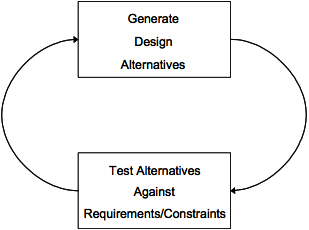
\includegraphics[width=0.60\textwidth]{GenerateTestCycle.png}
        \caption{The generate/test cycle, from \protect \citet{Hevner2004}}
        \label{GenerateTestCycle}
    \end{center}
\end{figure}

For the design process we look to \citet{Chen1990}, who proposes four activities that interact in the development of information systems( See figure \ref{multi} on page \pageref{multi}). 
The paper suggests using a multimethodological approach where one moves between different research activities: Theory building, experimentation, observation and systems development.
By using these different approaches we can hope that we will catch important facets that might otherwise have been missed or over looked.   

\begin{figure}[h]
    \begin{center}
        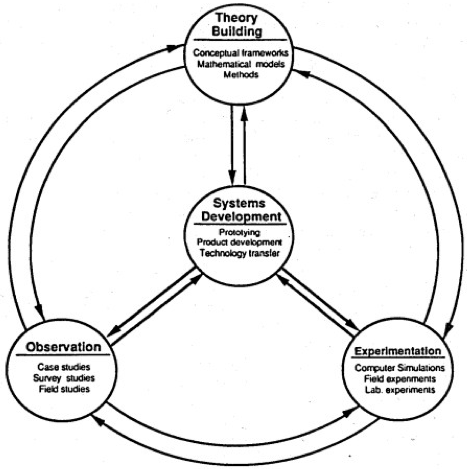
\includegraphics[width=0.60\textwidth]{MultiMethodological.png}
        \caption{A multimethodological approach to IS research, from \protect \citet{Chen1990}}
        \label{multi}
    \end{center}
\end{figure}